\documentclass{article}
\usepackage[utf8]{inputenc}
\usepackage{kotex}
\usepackage{amsmath}
\usepackage{kmath}
\usepackage{graphicx}
\usepackage{listings}
\usepackage{color}
\usepackage{subfigure}
\usepackage[a4paper,left=26mm,right=26mm,top=27mm,bottom=27mm]{geometry}


\title{Programming Language hw3}
\author{B811056 노이진}
\date{April 2021}

\begin{document}

\maketitle

코드가 가로로 길어서 페이지의 가로 길이를 길게 조절하였습니다.

\section{Yacc에 대한 설명}
Yacc(Yet Another Compiler-Compiler)란 문법을 확인해 프로그램의 계층 구조를 찾는 프로그램이다. \newline
야크와 렉스를 함께 이용하는데, 렉스에서는 정규 표현식에 맞는 토큰을 반환하고, 야크에서는 이를 이용해 파서를 만든다. 파싱은 lex에서 맞는 규칙에 따라 반환된 토큰에서 시작해 차례차례 reduce해서 진행한다. 이때 렉스에서 입력값을 토큰으로 나누는 것을 '어휘분석'이라고 하며, 이런 일을 하는 렉스는 어휘분석기가 된다. 그리고 토큰들이 수식인지, 문장인지, 선언문인지, 프로시저인지 판별하는 것을 '구문분석'이라고 하고 그 관계들의 규칙이 문법이다. 야크는 이때 구문분석기인 파서를 생성해주는 프로그램이다. 야크의 문법은 렉스와 비슷하다. 마찬가지로 정의절, 규칙절, 서브루틴절로 나눠져 있는데, 서브루틴절에서 yyparse()를 사용해야 파서를 생성할 수 있다. 이 때 파싱에러가 발생하면 yyerror()를 호출해 오류처리를 할 수 있다. 그리고 야크의 토큰 번호와 기타 변수의 정보가 "y.tap.h"에 저장되기 때문에 lex의 정의절에서 이를 꼭 include 해주어야 한다.

\section{Lex Code}
    기본적인 문법은 모두 pdf를 참고했으며 주석은 모두 //을 이용해 달았습니다.
\begin{lstlisting}[escapeinside=~~]
%{
#include <stdio.h>
#include "y.tab.h"

extern void yyerror(const char *);
int check_type(void);
%}
D [0-9]
L [a-zA-Z_]
H [a-fA-F0-9]
E [Ee][+-]?{D}+
FS (f|F|l|L)
IS (u|U|l|L)*
%%
"//".*\n	{ ; }       //~기존에 부족한 주석처리문을 추가해줌.~
"/*" { comment(); }
"#include".*\n	{ ; }       //~include를 받을 경우 아무것도 안하도록 새로운 규칙 추가~
#define.*\n	{ ; }       //~마찬가지로 define문을 처리하기 위한 규칙도 추가해줌.~
"auto" { return(AUTO); }
"break" { return(BREAK); }
"case" { return(CASE); }
"char" { return(CHAR); }
"const" { return(CONST); }
"continue" { return(CONTINUE); }
"default" { return(DEFAULT); }
"do" { return(DO); }
"double" {return(DOUBLE); }
"else" { return(ELSE); }
"enum" { return(ENUM); }
"extern" { return(EXTERN); }
"float" { return(FLOAT); }
"for" { return(FOR); }
"goto" { return(GOTO); }
"if" { return(IF); }
"int" { return(INT); }
"long" { return(LONG); }
"register" { return(REGISTER); }
"return" { return(RETURN); }
"short" { return(SHORT); }
"signed" { return(SIGNED); }
"sizeof" { return(SIZEOF); }
"static" { return(STATIC); }
"struct" { return(STRUCT); }
"switch" { return(SWITCH); }
"typedef" { return(TYPEDEF); }
"union" { return(UNION); }
"unsigned" { return(UNSIGNED); }
"void" { return(VOID); }
"volatile" { return(VOLATILE); }
"while" { return(WHILE); }
{L}({L}|{D})* { return(check_type()); }
0[xX]{H}+{IS}? { return(CONSTANT); }
0{D}+{IS}? { return(CONSTANT); }
{D}+{IS}? { return(CONSTANT); }
L?'(\\.|[^\\'])+' { return(CONSTANT); }
{D}+{E}{FS}? { return(CONSTANT); }
{D}*"."{D}+({E})?{FS}? { return(CONSTANT); }
{D}+"."{D}*({E})?{FS}? { return(CONSTANT); }
L?\"(\\.|[^\\"])*\" { return(STRING_LITERAL); }
"..." { return(ELLIPSIS);}
">>=" { return(RIGHT_ASSIGN);}
"<<=" { return(LEFT_ASSIGN);}
"+=" { return(ADD_ASSIGN); }
"-=" { return(SUB_ASSIGN); }
"*=" { return(MUL_ASSIGN); }
"/=" { return(DIV_ASSIGN); }
"%=" { return(MOD_ASSIGN); }
"&=" { return(AND_ASSIGN); }
"^=" { return(XOR_ASSIGN); }
"|=" { return(OR_ASSIGN); }
">>" { return(RIGHT_OP); }
"<<" { return(LEFT_OP); }
"++" { return(INC_OP); }
"--" { return(DEC_OP); }
"->" { return(PTR_OP); }
"&&" { return(AND_OP); }
"||" { return(OR_OP); }
"<=" { return(LE_OP); }
">=" { return(GE_OP); }
"==" { return(EQ_OP);}
"!=" { return(NE_OP); }
";" { return(';'); }
("{"|"<%") { return('{'); }
("}"|"%>") { return('}'); }
"," { return(','); }
":" { return(':'); }
"=" { return('='); }
"(" { return('('); }
")" { return(')'); }
("["|"<:") { return('['); }
("]"|":>") { return(']'); }
"." { return('.'); }
"&" { return('&'); }
"!" { return('!'); }
"~" { return('~'); }
"-" { return('-'); }
"+" { return('+'); }
"*" { return('*'); }
"/" { return('/'); }
"%" { return('%'); }
"<" { return('<'); }
">" { return('>'); }
"^" { return('^'); }
"|" { return('|'); }
"?" { return('?'); }
[ \t\v\n\f] { ;}
. { ; }
%%

int yywrap(void){
	return 1;
}

comment() //~주석을 print하지 않도록 putchar를 제거해줌.~
{
	char c, c1;
	loop:
	while ((c = input()) != '*' && c != 0) ;
	if ((c1 = input()) != '/' && c != 0){
		unput(c1);
		goto loop;
	}
}
//~필요없는 count()함수는 제거해줌.~

int check_type(){   //~typedef는 하지 않으니 주석 풀지 않음.~
	/*
	* pseudo code --- this is what it should check
	*
	* if (yytext == type_name)
	* return(TYPE_NAME);
	*
	* return(IDENTIFIER);
	*//*
	* it actually will only return IDENTIFIER
	*/
	return(IDENTIFIER);
}
\end{lstlisting}

\section{Yacc Code}
 기본적인 문법은 모두 pdf를 참고했으며 주석은 모두 //을 이용해 달았습니다.
\begin{lstlisting}[escapeinside=``]
%{
#include <stdio.h>
int ary[9] = {0,0,0,0,0,0,0,0,0};
int checkINT = 0;   //`int형 변수를 셀 때 이용할 checkINT 변수를 추가`
int checkCHAR = 0;  //`char형 변수를 셀 때 이용할 checkCHAR 변수를 추가`
%}
%token INCLUDE DEFINE
%token IDENTIFIER CONSTANT STRING_LITERAL SIZEOF
%token PTR_OP INC_OP DEC_OP LEFT_OP RIGHT_OP LE_OP GE_OP EQ_OP NE_OP
%token AND_OP OR_OP MUL_ASSIGN DIV_ASSIGN MOD_ASSIGN ADD_ASSIGN
%token SUB_ASSIGN LEFT_ASSIGN RIGHT_ASSIGN AND_ASSIGN
%token XOR_ASSIGN OR_ASSIGN TYPE_NAME
%token TYPEDEF EXTERN STATIC AUTO REGISTER
%token CHAR SHORT INT LONG SIGNED UNSIGNED FLOAT DOUBLE CONST VOLATILE VOID
%token STRUCT UNION ENUM ELLIPSIS
%token CASE DEFAULT IF ELSE SWITCH WHILE DO FOR GOTO CONTINUE BREAK RETURN
%start translation_unit
%%
primary_expression
	: IDENTIFIER
	| CONSTANT
	| STRING_LITERAL
	| '(' expression ')'
	;
postfix_expression
	: primary_expression
	| postfix_expression '[' expression ']' 
	| postfix_expression '(' ')' {ary[0] += 1;}
	//`printf()같은 함수를 나타내는 표현이므로 ary[0]에 1을 더해준다.`
	| postfix_expression '(' argument_expression_list ')' {ary[0] += 1; } 
	//`마찬가지로 func(a,b)같은 함수를 나타내는 표현이므로 ary[0]에 1을 더해준다.`
	| postfix_expression '.' IDENTIFIER {ary[1] += 1; }
	//`참조연산자 .을 나타내므로 operator count값을 +1한다.`
	| postfix_expression PTR_OP IDENTIFIER {ary[1] += 1; }
	//`마찬가지로 참조연산자 $-$$>$을 나타내므로 ary[1]++`
	| postfix_expression INC_OP {ary[1] += 1; }
	//`증감연산자 ++을 나타내므로 ary[1]++(후위)`
	| postfix_expression DEC_OP {ary[1] += 1; }
	//`증감연산자 $-$$-$을 나타내므로 ary[1]++(후위)`
	;
argument_expression_list
	: assignment_expression
	| argument_expression_list ',' assignment_expression
	;
unary_expression
	: postfix_expression 
	| INC_OP unary_expression {ary[1] += 1; }
	//`증감연산자 ++을 나타내므로 ary[1]++(전위)`
	| DEC_OP unary_expression {ary[1] += 1; }
	//`증감연산자 $-$$-$을 나타내므로 ary[1]++(전위)`
	| unary_operator cast_expression
	| SIZEOF unary_expression
	| SIZEOF '(' type_name ')'
	;
unary_operator
	: '&' 
	| '*' 
	| '+'
	| '-' 
	| '~' 
	| '!'
	;
cast_expression
	: unary_expression
	| '(' type_name ')' cast_expression {ary[1] += 1; }
	//`이 때 `cast_expression`은 `unary_expression`로, 그리고` postfix_expression, 
	primary_expression`로 reduce 되기 때문에 이는 (char) ad 같은`
	`경우를 말한다. 그리고 이는 cast연산자가 사용된 경우이므로 ary[1]을 +1 해준다.`
	;
multiplicative_expression
	: cast_expression
	| multiplicative_expression '*' cast_expression {ary[1] += 1; }
	//`산술연산자를 나타내므로 operator count값을 +1한다.`
	| multiplicative_expression '/' cast_expression {ary[1] += 1; }
	//`산술연산자를 나타내므로 operator count값을 +1한다.`
	| multiplicative_expression '%' cast_expression {ary[1] += 1; }
	//`산술연산자를 나타내므로 operator count값을 +1한다.`
	;
additive_expression
	: multiplicative_expression
	| additive_expression '+' multiplicative_expression {ary[1] += 1; }
	//`산술연산자를 나타내므로 operator count값을 +1한다.`
	| additive_expression '-' multiplicative_expression {ary[1] += 1; }
	//`산술연산자를 나타내므로 operator count값을 +1한다.`
	;
shift_expression
	: additive_expression
	| shift_expression LEFT_OP additive_expression {ary[1] += 1; }
	//`비트연산자를 나타내므로 operator count값을 +1한다.`
	| shift_expression RIGHT_OP additive_expression {ary[1] += 1; }
	//`비트연산자를 나타내므로 operator count값을 +1한다.`
	;
relational_expression
	: shift_expression
	| relational_expression '<' shift_expression {ary[1] += 1; }
	//`논리연산자를 나타내므로 operator count값을 +1한다.`
	| relational_expression '>' shift_expression {ary[1] += 1; }
	//`논리연산자를 나타내므로 operator count값을 +1한다.`
	| relational_expression LE_OP shift_expression {ary[1] += 1; }
	//`논리연산자를 나타내므로 operator count값을 +1한다.`
	| relational_expression GE_OP shift_expression {ary[1] += 1; }
	//`논리연산자를 나타내므로 operator count값을 +1한다.`
	;
equality_expression
	: relational_expression
	| equality_expression EQ_OP relational_expression {ary[1] += 1; }
	//`논리연산자를 나타내므로 operator count값을 +1한다.`
	| equality_expression NE_OP relational_expression {ary[1] += 1; }
	//`논리연산자를 나타내므로 operator count값을 +1한다.`
	;
and_expression
	: equality_expression
	| and_expression '&' equality_expression {ary[1] += 1; }
	//`비트연산자를 나타내므로 operator count값을 +1한다.`
	;
exclusive_or_expression
	: and_expression
	| exclusive_or_expression '^' and_expression {ary[1] += 1; }
	//`비트연산자를 나타내므로 operator count값을 +1한다.`
	;
inclusive_or_expression
	: exclusive_or_expression
	| inclusive_or_expression '|' exclusive_or_expression {ary[1] += 1;}
	//`비트연산자를 나타내므로 operator count값을 +1한다.`
	;
logical_and_expression
	: inclusive_or_expression
	| logical_and_expression AND_OP inclusive_or_expression {ary[1] += 1;}
	//`관계연산자를 나타내므로 operator count값을 +1한다.`
	;
logical_or_expression
	: logical_and_expression
	| logical_or_expression OR_OP logical_and_expression {ary[1] += 1;}
	//`관계연산자를 나타내므로 operator count값을 +1한다.`
	;
conditional_expression
	: logical_or_expression
	| logical_or_expression '?' expression ':' conditional_expression
	//`삼항연산자이므로 카운팅하지 않음.`
	;
assignment_expression
	: conditional_expression
	| unary_expression assignment_operator assignment_expression 
	{ary[1] += 1;}
	//assignment_operator`가 사용될 경우인데, 이는 이항연산자의 사용을 의미하므로` 
	`operator count값을 +1한다.`
	;
assignment_operator
	: '='
	| MUL_ASSIGN 
	| DIV_ASSIGN 
	| MOD_ASSIGN 
	| ADD_ASSIGN 
	| SUB_ASSIGN 
	| LEFT_ASSIGN 
	| RIGHT_ASSIGN 
	| AND_ASSIGN 
	| XOR_ASSIGN 
	| OR_ASSIGN 
	;
expression
	: assignment_expression
	| expression ',' assignment_expression
	;
constant_expression
	: conditional_expression
	;
declaration
	: declaration_specifiers ';'
	| declaration_specifiers init_declarator_list ';' 
	{if(checkCHAR == 1) ary[3]++; if(checkINT == 1) ary[2]++; 
	checkCHAR = 0; checkINT = 0; }
	//`예를 들어 int 변수의 개수를 셀 때, 앞의 int는 type spcifier에서 declaration specifiers로`
	`reduce되고, 뒷부분은 IDENTIFER, direct declarator, declarator, init declarator, init declarator 로` 
	`reduce되서 둘과 ';'이 합쳐져 declaration으로 reduce된다.`
	`그 때 int a = 1; 같은 변수선언이 완성되는데 이 때 int를 count하는 값을`
	`+1하고, 변수 선언이 완성됐으므로 checkINT변수를 다시 0으로 초기화해서 다음 변수 선언 때`
	`잘못세는 일이 없도록 해야한다. char 변수세는 방법도 완전히 동일하다.`
	`check변수는 원하는 type을 만났을 때 1로 바뀌도록 type specifier에서 설정한다. `
	;
declaration_specifiers
	: storage_class_specifier
	| storage_class_specifier declaration_specifiers
	| type_specifier
	| type_specifier declaration_specifiers
	| type_qualifier
	| type_qualifier declaration_specifiers
	;
init_declarator_list
	: init_declarator
	| init_declarator_list ',' init_declarator 
	{if(checkCHAR == 1) ary[3]++; if(checkINT == 1) ary[2]++; }
	//`int a,b와 같은 경우, int를 1개가 아니라 2개로 세줘야하므로 사이에 콤마가 있으면 check변수에` 
	`맞는 변수의 count값을 +1해준다. 이때 init declarator list는 콤마로 init declarator로 연결할 수` 
	`있으므로 콤마가 있을 때마다 count하는 값이 +1되서 정상적으로 셀 수 있다.`
	;
init_declarator
	: declarator
	| declarator '=' initializer {ary[1] += 1;}
	//`=을 이용해 표현한 경우이므로 대입연산자가 사용된 경우이다. 따라서 ary[1]++해준다.`
	;
storage_class_specifier
	: TYPEDEF
	| EXTERN
	| STATIC
	| AUTO
	| REGISTER
	;
type_specifier
	: VOID
	| CHAR { checkCHAR = 1; }   //`char을 발견하면 checkCHAR을 1로 바꿔준다.`
	| SHORT
	| INT { checkINT = 1; }   //`int를 발견하면 checkINT을 1로 바꿔준다.`
	| LONG
	| FLOAT
	| DOUBLE
	| SIGNED
	| UNSIGNED
	| struct_or_union_specifier
	| enum_specifier
	| TYPE_NAME
	;
struct_or_union_specifier
	: struct_or_union IDENTIFIER '{' struct_declaration_list '}'
	| struct_or_union '{' struct_declaration_list '}'
	| struct_or_union IDENTIFIER
	;
struct_or_union
	: STRUCT
	| UNION
	;
struct_declaration_list
	: struct_declaration
	| struct_declaration_list struct_declaration
	;
struct_declaration
	: specifier_qualifier_list struct_declarator_list ';'
	;
specifier_qualifier_list
	: type_specifier specifier_qualifier_list
	| type_specifier
	| type_qualifier specifier_qualifier_list
	| type_qualifier
	;
struct_declarator_list
	: struct_declarator
	| struct_declarator_list ',' struct_declarator
	;
struct_declarator
	: declarator
	| ':' constant_expression
	| declarator ':' constant_expression
	;
enum_specifier
	: ENUM '{' enumerator_list '}'
	| ENUM IDENTIFIER '{' enumerator_list '}'
	| ENUM IDENTIFIER
	;
enumerator_list
	: enumerator
	| enumerator_list ',' enumerator
	;
enumerator
	: IDENTIFIER
	| IDENTIFIER '=' constant_expression {ary[1] += 1; }
	//`=을 이용해 표현한 경우이므로 대입연산자가 사용된 경우이다. 따라서 ary[1]++해준다.`
	;
type_qualifier
	: CONST
	| VOLATILE
	;
declarator
	: pointer direct_declarator
	| direct_declarator
	;
direct_declarator
	: IDENTIFIER
	| '(' declarator ')'
	| direct_declarator '[' constant_expression ']' {ary[5] += 1;}
	//`a[40]과 같은 array를 표현하는 것이다. 따라서 ary[5]++ 해줬다.`
	| direct_declarator '[' ']' {ary[5] += 1;}
	//`a[] = {...}와 같은 array를 표현하는 것이다. 따라서 ary[5]++ 해줬다.`
	| direct_declarator '(' parameter_type_list ')' 
	{checkCHAR = 0; checkINT = 0; }
	//`func(int i, char c)와 같은 함수 선언을 표현하는 것이다. 함수값은 정의할 때만 세므로 +1해주지`
	`않고, 이 경우 parameter들의 type들이 이미 count된 후이므로 check변수들을 0으로 초기화해 다음 `
	`int나 char을 셀 때 영향을 주지 않도록 한다.`
	| direct_declarator '(' identifier_list ')'
	| direct_declarator '(' ')'
	;
pointer
	: '*' {ary[4] += 1;}
	//`포인터이므로 ary[4]++`
	| '*' type_qualifier_list {ary[4] += 1;}
	//`포인터이므로 ary[4]++`
	| '*' pointer {ary[4] += 1;}
	//`포인터이므로 ary[4]++`
	| '*' type_qualifier_list pointer {ary[4] += 1;}
	//`포인터이므로 ary[4]++`
	;
type_qualifier_list
	: type_qualifier
	| type_qualifier_list type_qualifier
	;
parameter_type_list
	: parameter_list 
	| parameter_list ',' ELLIPSIS
	;
parameter_list
	: parameter_declaration 
	| parameter_list ',' parameter_declaration 
	;
parameter_declaration
	: declaration_specifiers declarator 
	{if(checkCHAR == 1) ary[3]++; if(checkINT == 1) ary[2]++; }
	//`함수의 parameter들에서 int와 char개수를 세기 위해 check변수를 확인하고`
	`+1을 해주었다.`
	| declaration_specifiers abstract_declarator 
	{if(checkCHAR == 1) ary[3]++; if(checkINT == 1) ary[2]++; }
	//`함수의 parameter들에서 int와 char개수를 세기 위해 check변수를 확인하고`
	`+1을 해주었다.`
	| declaration_specifiers
	;
identifier_list
	: IDENTIFIER
	| identifier_list ',' IDENTIFIER
	;
type_name
	: specifier_qualifier_list
	| specifier_qualifier_list abstract_declarator
	;
abstract_declarator
	: pointer
	| direct_abstract_declarator
	| pointer direct_abstract_declarator
	;
direct_abstract_declarator
	: '(' abstract_declarator ')'
	| '[' ']'
	| '[' constant_expression ']'
	| direct_abstract_declarator '[' ']' 
	| direct_abstract_declarator '[' constant_expression ']'
	| '(' ')'
	| '(' parameter_type_list ')'
	| direct_abstract_declarator '(' ')' 
	| direct_abstract_declarator '(' parameter_type_list ')' 
	{checkCHAR = 0; checkINT = 0; } 
	//`parameter들의 type들이 이미 count된 후 이므로 check변수들을 0으로 초기화 해`
	`다음 int나 char을 셀 때 영향을 주지 않도록 한다.`
	;
initializer
	: assignment_expression
	| '{' initializer_list '}'
	| '{' initializer_list ',' '}'
	;
initializer_list
	: initializer
	| initializer_list ',' initializer
	;
statement
	: labeled_statement
	| compound_statement
	| expression_statement
	| selection_statement
	| iteration_statement
	| jump_statement
	;
labeled_statement
	: IDENTIFIER ':' statement
	| CASE constant_expression ':' statement
	| DEFAULT ':' statement
	;
compound_statement
	: '{' '}'
	| '{' statement_list '}'
	| '{' declaration_list '}'
	| '{' declaration_list statement_list '}'
	;
declaration_list
	: declaration
	| declaration_list declaration
	;
statement_list
	: statement
	| statement_list statement
	| statement_list declaration_list statement
	//`그 전에는 변수가 전방선언만 가능했던 이유는 statement list가 그렇게`
	   `설정되어 있었기 때문이다. 따라서 declaration list가 statement list 뒤에 오고 그 뒤에` 
	   `statement가 와서 자유선언이 가능하도록 세번째 줄의 새로운 규칙을 추가했다.`
	;
expression_statement
	: ';'
	| expression ';'
	;
selection_statement
	: IF '(' expression ')' statement {ary[6] += 1;}
	//`선택문이므로 ary[6]을 ++해주었다. 다만 else,if else문은 conflict만 일으키고`
	`선택문을 세는 데에서 제외되므로 아예 빼버렸다.`
	| SWITCH '(' expression ')' statement {ary[6] += 1;}
	//`선택문이므로 ary[6]을 ++해주었다.`
	;
iteration_statement
	: WHILE '(' expression ')' statement {ary[7] += 1;}
	//`반복문 while문이므로 ary[7]을 ++해주었다.`
	| DO statement WHILE '(' expression ')' ';' {ary[7] += 1;}
	//`반복문 do while문이므로 ary[7]을 ++해주었다.`
	| FOR '(' expression_statement expression_statement ')' statement 
	{ary[7] += 1;}
	//`반복문 for문이므로 ary[7]을 ++해주었다. 이 때는 for(i = 0; i < N ; i++)이 있을 때`
	`i++(expression)이 빠진 for문`
	| FOR '(' expression_statement expression_statement expression ')' statement
	{ary[7] += 1;}
	//`반복문 for문이므로 ary[7]을 ++해주었다. 이 때는 우리가 아는 정상 for문`
	;
jump_statement
	: GOTO IDENTIFIER ';'
	| CONTINUE ';'
	| BREAK ';'
	| RETURN ';' {ary[8] += 1;}
	//`return문이므로 ary[7]을 ++해주었다. 이때는 반환하는 값 없음`
	| RETURN expression ';' {ary[8] += 1;}
	//`return문이므로 ary[7]을 ++해주었다. 이때는 return high;처럼 expression 반환`
	;
translation_unit
	: external_declaration
	| translation_unit external_declaration
	;
external_declaration
	: function_definition 
	| declaration
	;
function_definition
	: declaration_specifiers declarator declaration_list compound_statement 
	{ ary[0] += 1; checkCHAR = 0; checkINT = 0; }
	| declaration_specifiers declarator compound_statement 
	{ ary[0] += 1; checkCHAR = 0; checkINT = 0; } 
	| declarator declaration_list compound_statement 
	{ ary[0] += 1; checkCHAR = 0; checkINT = 0; } 
	| declarator compound_statement 
	{ ary[0] += 1; checkCHAR = 0; checkINT = 0; } 
	;   //`함수가 정의될 때마다 함수 count하는 값을 +1해주고, 무조건 check변수들을 초기화하게` 
	    `했다. int나 char형을 반환하는 함수일 경우, int나 char을 count하는 값을 +1해주면 안되므로`
	    `하지 않았다. 또한 그것을 방지하기 위해 type specifier에서 int,char를 count하는 값을 +1`
	    `해주지않고 check변수를 만들어 어디서 파싱되는지 파싱트리를 그려 그 부분마다 count`
	    `했다. 무조건 check변수를 초기화하는 이유는 혹시 초기화 되지 않아 check변수가`
	    `1으롤 남아있어 count되는 경우를 막기위해서 그냥 함수 때마다 초기화 하도록 했다. `
	    `함수가 끝났을 때는 어차피 언제나 새로운 변수나 파리미터를 받기 위한 준비가 `
	    `되어있어야 하기 때문이다.`
%%

int main(void)
{
	yyparse();
	printf("function = %d\n", ary[0]);
	printf("operator = %d\n", ary[1]);
	printf("int = %d\n", ary[2]);
	printf("char = %d\n", ary[3]);
	printf("pointer = %d\n", ary[4]);
	printf("array = %d\n", ary[5]);
	printf("selection = %d\n", ary[6]);
	printf("loop = %d\n", ary[7]);
	printf("return = %d\n", ary[8]);
	return 0;
}

void yyerror(const char *str)
{
	fprintf(stderr, "error: %s\n", str);
}


\end{lstlisting}

\section{리눅스 환경 구축}
리눅스 서버가 닫혀있는 동안 리눅스 환경을 구축해서 yacc를 실행해 보았습니다.\newline
virtual box와 ubuntu를 이용했습니다.

\begin{figure}[ht]
\centering
    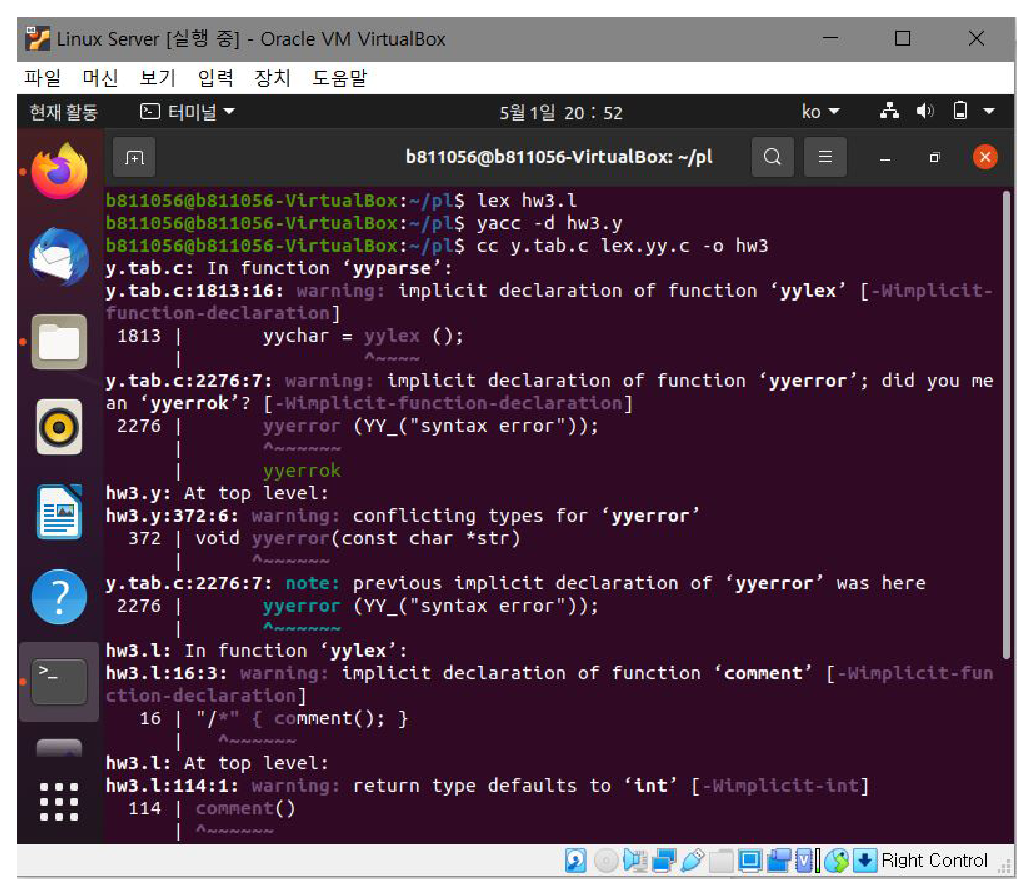
\includegraphics[width=.8\linewidth]{linux1}  
\end{figure}

\begin{figure}[ht]
\centering
   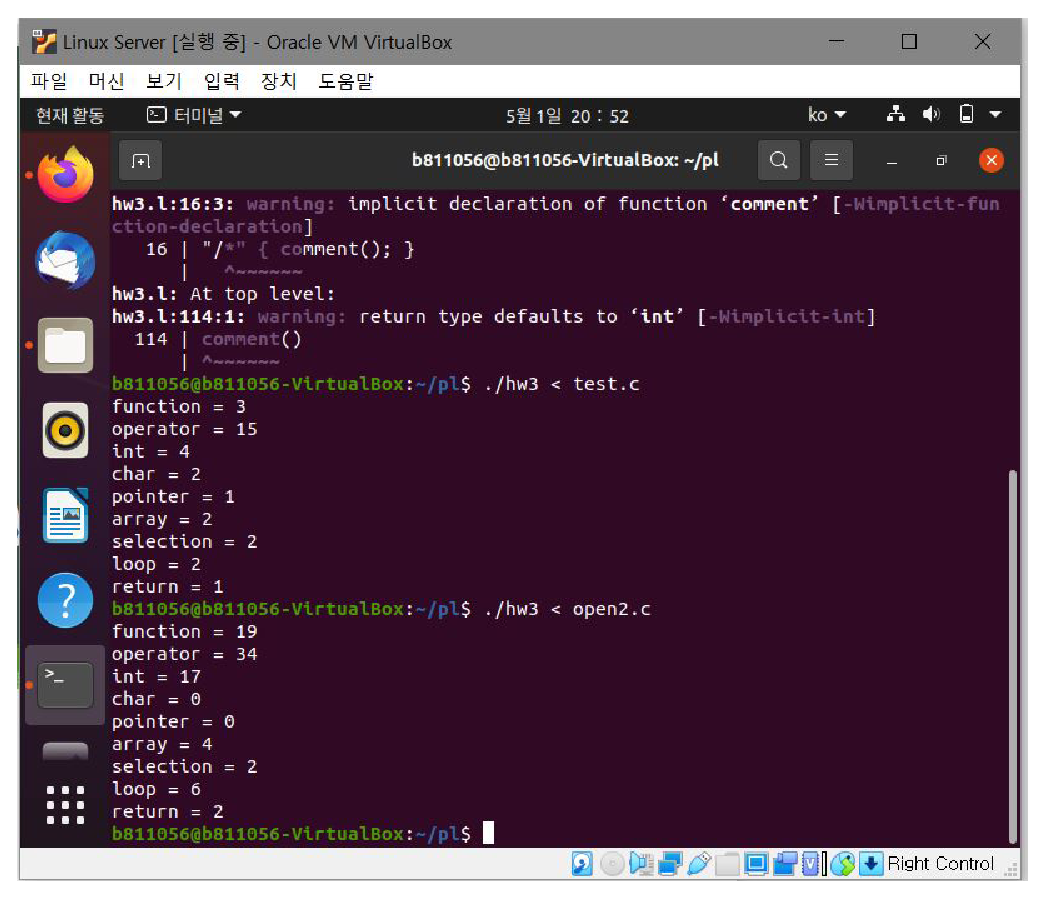
\includegraphics[width=.8\linewidth]{linux2}
\end{figure}

\begin{figure}[ht]
\centering
   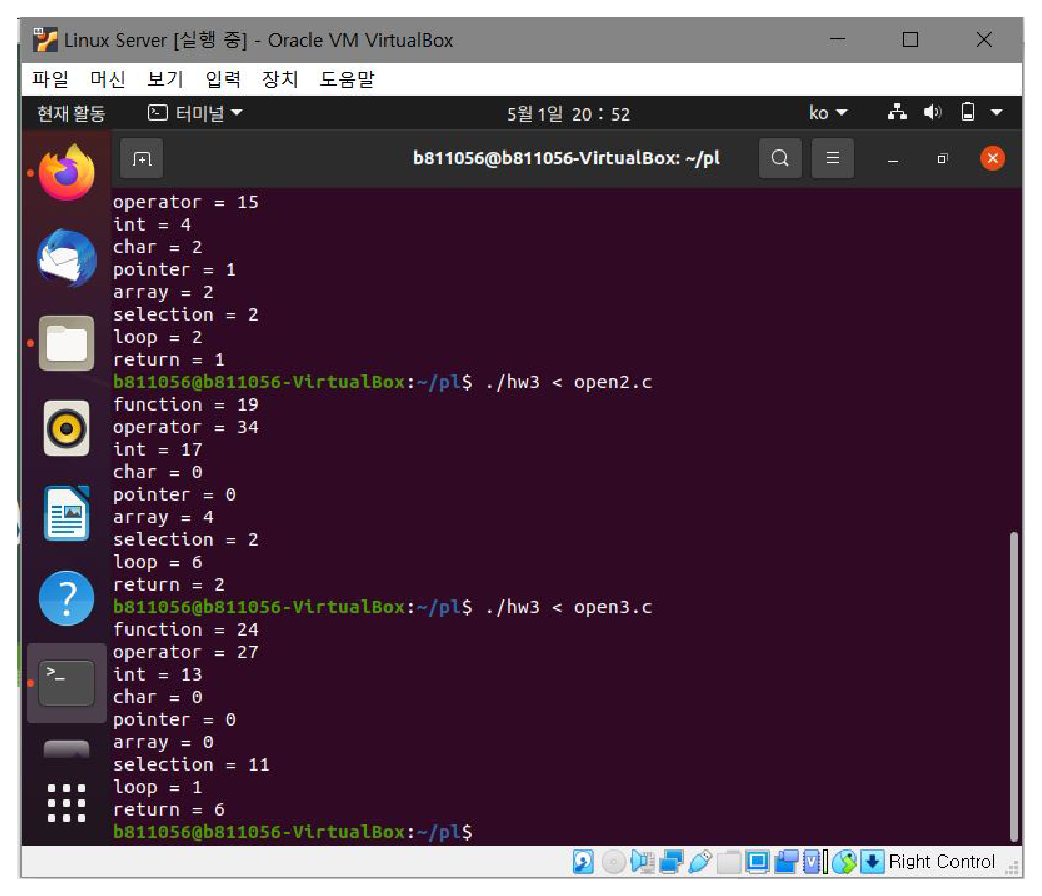
\includegraphics[width=.8\linewidth]{linux3}
\end{figure}

\end{document}
